\section{Measurement of Capacitors}
The measurement of capacitor values are done as separate task by measurement of load time
after all other measurements. 
The original software of Markus F. did this with a program loop, which reads the corresponding digital input
pin until a switch occured and count the loop cycles.
This has the handicap, that the resolution of time measurement is limited by the
time consumption of one loop cycle.
This usually was done in all six combinations for all three probe pins. 
The actual software uses two different ways to get the load time in only
three combinations for the three probe pins. The positive side is now always the
higher probe number. Only if capacity is measured parallel with a diode, the
polarity can be in the other order.

\subsection{Discharging of Capacitors}
You should always discharge the capacitor before connecting it to the tester.
The tester additionally discharge the capacitor before any measurement.
If the voltage is below 1300mV, the capacitor is shortened by the output pins of the connected ADC port (Port C).
I~believe that this is legal because every output port has a built in resistance of about \(20\Omega\).
The data sheet Figure 149 (page 258) \cite{ATmega8} shows voltage drop of output pins up to 2V.
Of course I can not guaranty, that no damage can occur. 
I~have tested the function with a 15mF Capacitor many times and I~have never noticed any problem.
The current should be below the specified limit of 40mA and is reduced fast by discharging.
Off course damage can occur if you do not discharge a (high voltage) capacitor before connecting it to your tester.

\subsection{Measurement of big Capacitors}
\label{sec:bigcap}
One side of the capacitor is connected to GND. The other side of the capacitor is connected with the
\(680\Omega\) resistor to VCC for a period of 10ms. Afterwards this probe pin is switched to Input (High Impedance).
After this 10 ms current pulse the voltage of the capacitor is measured without any current. If the voltage has not
reached a minimal value of 300mV, the load pulse is repeated up to 499 times.
If after 127 pulses a minimum voltage of 75mV is not reached (about 2s), further load is stopped, because never
the 300mV can be reached with the remaining load pulses.
Figure~\ref{fig:bigcap} shows the three phases of measuring the capacity value of a capacitor.
The value of the capacity is then computed with the count of load pulses and the reached load voltage from a table.
The table contains  the factors to get the capacity in nF units from load time and the reached voltage
with a spacing of 25mV.
Interim value of voltage will be interpolated.

\begin{figure}[H]
\centering

\includegraphics[]{../FIG/Bigcap.eps}
\caption{discharge a capacitor and load with 10ms load pulses until voltage reach a value of 300mV}
\label{fig:bigcap}
\end{figure}
As a result of the low load voltage, the measurement is much faster than the initial software version,
 because this advantage works also on discharging. So bigger capacitors can be measured.
Furthermore a diode, which is parallel connected to the capacitor don´t disturb the measurement in most cases,
because the flux voltage of most diodes is not reached.
Figure~\ref{pic:c229} shows the charge and discharge for a \(229\mu F\) capacitor.
The flat top of diagram from load end to discharge begin is caused by the measuring and computing time of the ATmega.
Figure~\ref{pic:c5mF} shows the same measurement for a~\(5mF\) capacitor,
notice how the time for measurement is grown to about 1.5 seconds inclusive the discharge. 
The last example shows the capacity measuring of a~\(15mF\) capacitor in Figure~\ref{pic:c15mF}

\begin{figure}[H]
  \begin{subfigure}[b]{9cm}
    \centering
    \includegraphics[width=9cm]{../PNG/charge_229uF.png}
    \caption{\(229\mu F\) Capacitor}
    \label{pic:c229}
  \end{subfigure}
  ~
  \begin{subfigure}[b]{9cm}
    \centering
    \includegraphics[width=9cm]{../PNG/charge_5mF.png}
    \caption{\(5mF\) Capacitor}
    \label{pic:c5mF}
  \end{subfigure}
  \caption{Charge and discharge of big Capacitors for measuring}
\end{figure}

\begin{figure}[H]
  \centering
    \includegraphics[]{../PNG/charge_15mF.png}
  \caption{Charge and discharge of a \(15mF\) Capacitor for measuring}
  \label{pic:c15mF}
\end{figure}

\subsection{Measurement of small Capacitors}
If the first 10 ms load pulse has overloaded the capacitor, another technique of measurement is used.
The ATmega processor has a build in 16-Bit counter, which can operate at the full clock rate (1MHz or 8MHz).
This counter has also the feature to save his counter value by a external event.
This event can be built by the output of the comparator. 
The comparator can operate with any ADC input pin and the band gap reference.
Figure~\ref{fig:comparat} shows a simplified diagram of the measurement situation.
So I discharge the capacitor, prepare the comparator to the proper pin input, start the counter at 0 and
start immediately the charging of the capacitor with one side connected to GND and the other side connected with
the \(470k\Omega\) resistor to VCC.
Now I check within a program loop, if the counter flags signals a overflow event or a input capture (external) event.
I count the overflow events until I detect the input capture event.
In this case I stop the counter and check if I must count a additional overflow,
because the counter can't be stopped by the input capture event.


The input capture counter and the overflow counter built together the total time,
from which I subtract a predefined experimental find out constant or a value found by the last selftest to eliminate the measurement offset. 
I don't know, if the experimental find out constant must be adapted to other printed circuit boards.
The actual software can use a table with the theoretical  dependency of the load time in respect to the comparator voltage.
The table is spaced in 50mV steps and will be interpolated according to the actual reference voltage. 
This table will only be acticated with the Makefile option WITH\_AUTO\_REF.
I noticed that the reference voltage is permanently somewhat to low,
 so that you can choose an offset with the Makefile option REF\_C\_KORR.
The measured reference voltage will then be corrected (added) by your value (mV units).
If option WITH\_AUTO\_REF is not used, the reference voltages of ATmega8, ATmega88, ATmega168 and ATmega328
are applied as noted in the data sheets~\cite{ATmega8}~\cite{ATmega168}. 
A sample measurement of this type is shown in figure~\ref{pic:c22uF}.
The measurement time for the \(22 \mu F\) capacitor is above 2.6s because the \(470k\Omega\) is
used for charging. But discharging is in this case much faster than charging.

\begin{figure}[H]
\centering

\includegraphics[]{../FIG/Comparat.eps}
\caption{measurement little capacity values with comparator}
\label{fig:comparat}
\end{figure}

\begin{figure}[H]
  \centering
    \includegraphics[]{../PNG/charge_22uF.png}
  \caption{Charge and discharge of a \(22\mu F\) Capacitor for measuring}
  \label{pic:c22uF}
\end{figure}


In principle this technique of measurement can also be done with the \(680\Omega\) resistor, but 
because the ADC can't be used if the comparator is working, I have no chance to monitor the
load voltage until the comparator is stopped. If a undetected diode is parallel connected with
the capacitor, the load current of the capacitor can be absorbed by the diode (threshold voltage) and
the band-gap voltage will never be reached.
The method taken in actual software for big capacitors in section~\ref{sec:bigcap}
avoids this conceptual bug.

\subsection{Results of Capacitor measurement}
The results of my measurements is shown if figure~\ref{fig:mega8cap} for ATmega8 processor without and 
with the AUTOSCALE\_ADC option. Additionally some values of original software are shown with a correction factor
of 0.88 (-12\%).
The results of the measurement of the same capacitors for a ATmega168 is shown in figure~\ref{fig:mega168cap}.
The reference for the error computing is the measurement of a PeakTech 2170 RCL-meter, not the printed value
of the parts.
A part of the relative high measurement difference is caused be the too high measurement frequency for big
electrolytical capacitors. On the other side the bad quality factor of the electrolytical capacitors may cause
another percentage.

\begin{figure}[H]
\centering
\input{../GNU/Mega8cap}
\caption{Error in \% for capacitor measurements with ATmega8 }
\label{fig:mega8cap}
\end{figure}

\begin{figure}[H]
\centering
\input{../GNU/Mega168cap}
\caption{Error in \% for capacitor measurements with ATmega168 }
\label{fig:mega168cap}
\end{figure}

Figure~\ref{fig:capcompare} illustrates, how difficult is it to choose the right base for the capacity measurement.
All measurement results are compared with the printed value of the capacitors.
The gradient ,,Multimeter'' shows the differences of the Peaktech~3315 Multimeter results.
The next gradient ,,LCR'' shows the differences of the Peaktech~2170 LCR-Meter results, which is taken from best frequency approach.
To compare this results to the results of a ATmega168 equipped Transistor-Tester the gradient ,,ATmega168as'' is also shown.
I beleave, that this errors are not real measurement errors of the particular equipment, because the printed value are
also not the real capacity value of the capacitors.

\begin{figure}[H]
\centering
% GNUPLOT: LaTeX picture with Postscript
\begingroup
  \makeatletter
  \providecommand\color[2][]{%
    \GenericError{(gnuplot) \space\space\space\@spaces}{%
      Package color not loaded in conjunction with
      terminal option `colourtext'%
    }{See the gnuplot documentation for explanation.%
    }{Either use 'blacktext' in gnuplot or load the package
      color.sty in LaTeX.}%
    \renewcommand\color[2][]{}%
  }%
  \providecommand\includegraphics[2][]{%
    \GenericError{(gnuplot) \space\space\space\@spaces}{%
      Package graphicx or graphics not loaded%
    }{See the gnuplot documentation for explanation.%
    }{The gnuplot epslatex terminal needs graphicx.sty or graphics.sty.}%
    \renewcommand\includegraphics[2][]{}%
  }%
  \providecommand\rotatebox[2]{#2}%
  \@ifundefined{ifGPcolor}{%
    \newif\ifGPcolor
    \GPcolortrue
  }{}%
  \@ifundefined{ifGPblacktext}{%
    \newif\ifGPblacktext
    \GPblacktexttrue
  }{}%
  % define a \g@addto@macro without @ in the name:
  \let\gplgaddtomacro\g@addto@macro
  % define empty templates for all commands taking text:
  \gdef\gplbacktext{}%
  \gdef\gplfronttext{}%
  \makeatother
  \ifGPblacktext
    % no textcolor at all
    \def\colorrgb#1{}%
    \def\colorgray#1{}%
  \else
    % gray or color?
    \ifGPcolor
      \def\colorrgb#1{\color[rgb]{#1}}%
      \def\colorgray#1{\color[gray]{#1}}%
      \expandafter\def\csname LTw\endcsname{\color{white}}%
      \expandafter\def\csname LTb\endcsname{\color{black}}%
      \expandafter\def\csname LTa\endcsname{\color{black}}%
      \expandafter\def\csname LT0\endcsname{\color[rgb]{1,0,0}}%
      \expandafter\def\csname LT1\endcsname{\color[rgb]{0,1,0}}%
      \expandafter\def\csname LT2\endcsname{\color[rgb]{0,0,1}}%
      \expandafter\def\csname LT3\endcsname{\color[rgb]{1,0,1}}%
      \expandafter\def\csname LT4\endcsname{\color[rgb]{0,1,1}}%
      \expandafter\def\csname LT5\endcsname{\color[rgb]{1,1,0}}%
      \expandafter\def\csname LT6\endcsname{\color[rgb]{0,0,0}}%
      \expandafter\def\csname LT7\endcsname{\color[rgb]{1,0.3,0}}%
      \expandafter\def\csname LT8\endcsname{\color[rgb]{0.5,0.5,0.5}}%
    \else
      % gray
      \def\colorrgb#1{\color{black}}%
      \def\colorgray#1{\color[gray]{#1}}%
      \expandafter\def\csname LTw\endcsname{\color{white}}%
      \expandafter\def\csname LTb\endcsname{\color{black}}%
      \expandafter\def\csname LTa\endcsname{\color{black}}%
      \expandafter\def\csname LT0\endcsname{\color{black}}%
      \expandafter\def\csname LT1\endcsname{\color{black}}%
      \expandafter\def\csname LT2\endcsname{\color{black}}%
      \expandafter\def\csname LT3\endcsname{\color{black}}%
      \expandafter\def\csname LT4\endcsname{\color{black}}%
      \expandafter\def\csname LT5\endcsname{\color{black}}%
      \expandafter\def\csname LT6\endcsname{\color{black}}%
      \expandafter\def\csname LT7\endcsname{\color{black}}%
      \expandafter\def\csname LT8\endcsname{\color{black}}%
    \fi
  \fi
  \setlength{\unitlength}{0.0500bp}%
  \begin{picture}(7200.00,5040.00)%
    \gplgaddtomacro\gplbacktext{%
      \csname LTb\endcsname%
      \put(682,704){\makebox(0,0)[r]{\strut{}-4}}%
      \csname LTb\endcsname%
      \put(682,1074){\makebox(0,0)[r]{\strut{}-3}}%
      \csname LTb\endcsname%
      \put(682,1444){\makebox(0,0)[r]{\strut{}-2}}%
      \csname LTb\endcsname%
      \put(682,1814){\makebox(0,0)[r]{\strut{}-1}}%
      \csname LTb\endcsname%
      \put(682,2184){\makebox(0,0)[r]{\strut{} 0}}%
      \csname LTb\endcsname%
      \put(682,2554){\makebox(0,0)[r]{\strut{} 1}}%
      \csname LTb\endcsname%
      \put(682,2925){\makebox(0,0)[r]{\strut{} 2}}%
      \csname LTb\endcsname%
      \put(682,3295){\makebox(0,0)[r]{\strut{} 3}}%
      \csname LTb\endcsname%
      \put(682,3665){\makebox(0,0)[r]{\strut{} 4}}%
      \csname LTb\endcsname%
      \put(682,4035){\makebox(0,0)[r]{\strut{} 5}}%
      \csname LTb\endcsname%
      \put(682,4405){\makebox(0,0)[r]{\strut{} 6}}%
      \csname LTb\endcsname%
      \put(682,4775){\makebox(0,0)[r]{\strut{} 7}}%
      \csname LTb\endcsname%
      \put(814,484){\makebox(0,0){\strut{}10p}}%
      \csname LTb\endcsname%
      \put(1413,484){\makebox(0,0){\strut{}100p}}%
      \csname LTb\endcsname%
      \put(2012,484){\makebox(0,0){\strut{}1n}}%
      \csname LTb\endcsname%
      \put(2611,484){\makebox(0,0){\strut{}10n}}%
      \csname LTb\endcsname%
      \put(3210,484){\makebox(0,0){\strut{}100n}}%
      \csname LTb\endcsname%
      \put(3809,484){\makebox(0,0){\strut{}1u}}%
      \csname LTb\endcsname%
      \put(4407,484){\makebox(0,0){\strut{}10u}}%
      \csname LTb\endcsname%
      \put(5006,484){\makebox(0,0){\strut{}100u}}%
      \csname LTb\endcsname%
      \put(5605,484){\makebox(0,0){\strut{}1m}}%
      \csname LTb\endcsname%
      \put(6204,484){\makebox(0,0){\strut{}10m}}%
      \csname LTb\endcsname%
      \put(6803,484){\makebox(0,0){\strut{}100m}}%
      \put(176,2739){\rotatebox{-270}{\makebox(0,0){\strut{}Error / Percent}}}%
      \put(3808,154){\makebox(0,0){\strut{}Capacity value / F}}%
      \put(3808,4665){\makebox(0,0){\strut{}}}%
    }%
    \gplgaddtomacro\gplfronttext{%
      \csname LTb\endcsname%
      \put(2266,4602){\makebox(0,0)[r]{\strut{}Multimeter}}%
      \csname LTb\endcsname%
      \put(2266,4382){\makebox(0,0)[r]{\strut{}LCR}}%
      \csname LTb\endcsname%
      \put(2266,4162){\makebox(0,0)[r]{\strut{}Mega168as}}%
    }%
    \gplbacktext
    \put(0,0){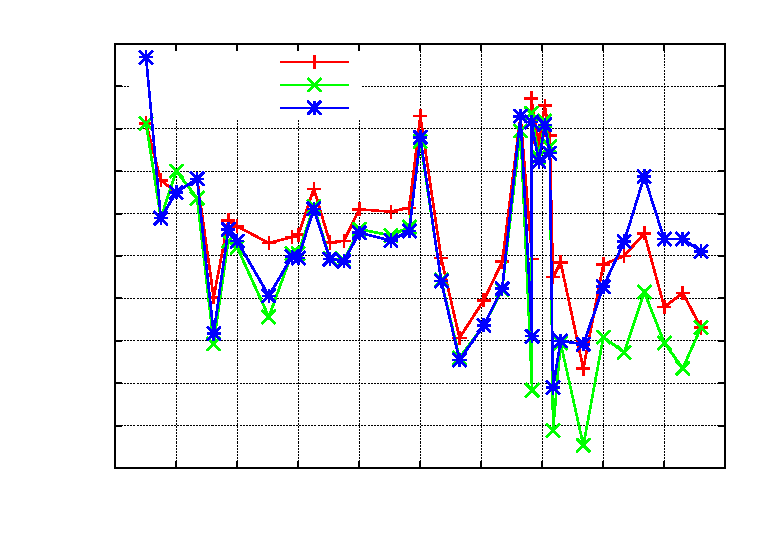
\includegraphics{../GNU/capcompare}}%
    \gplfronttext
  \end{picture}%
\endgroup

\caption{Comparison of capacity measurement results of Multimeter, LCR-meter and ATmega168}
\label{fig:capcompare}
\end{figure}

The differences of measurements of three different ATmega168 processors are shown in figure~\ref{fig:mega168all} .
In this case the results of the LCR~meter is taken as base of comparison.
The same results of three different ATmega168A processors are shown in figure~\ref{fig:mega168Aall} and
three different ATmega168PA processors are shown in figure~\ref{fig:mega168PAall}.
At this only the zero value of the capacity measurement of 39pF is respected, all other facility to correct the results are
not used.
This zero value includes the 2-3pF, which are caused by the 12 cm long cable with the clips.
The board layout can cause a different zero value, I have fixed this zero value with the board ''DG2BRS V 5.2.1''.

\begin{figure}[H]
\centering
\input{../GNU/Mega168all}
\caption{capacity measurement error of three ATmega168, not calibrated}
\label{fig:mega168all}
\end{figure}

\begin{figure}[H]
\centering
\input{../GNU/Mega168Aall}
\caption{capacity measurement error of three ATmega168A, not calibrated}
\label{fig:mega168Aall}
\end{figure}

\begin{figure}[H]
\centering
\input{../GNU/Mega168PAall}
\caption{capacity measurement error of three ATmega168PA, not calibrated}
\label{fig:mega168PAall}
\end{figure}

To get the best accuracy you must adapt the software to the individual characteristic of your ATmega exemplar.
For this you can set a correction voltage REF\_C\_KORR for the comparator, which will be used for measurement of little capacity values.
A correction of 1~mV will reduce the measurement results to 0.11~\% .
For big capacity values you can specify with the per mill value C\_H\_KORR, how much your capacity values are measured too big.
Because the capacitors with big values are most electrolytic capacitors with worse quality factor, the measurement of
the capacity value is difficult. So it is also extra difficult to get the difference to the real value of a capacitor.

Especially with the ATmega168 processors I have noticed a anomaly of measurement results of little capacity values,
which depend on the slew rate of the voltage during loading of the capacitor.
Figure~\ref{fig:mega168optcap} shows the error of the capacity measurement when only the zero value is respected
(168-3-A), with correction factor for little capacitors REF\_C\_KORR=66 as well as the correction factor for big
capacitors C\_H\_KORR=5 (168-3-B), plus additional as gradient 168-3-C  with a model of the slew rate dependency of little capacitor 
measurements (COMP\_SLEW1=4000 und COMP\_SLEW2=220). Also the self-discharge of big capacitors is respected with gradient 168-3-C.
The component with the slew rate dependent value is computed with \(\frac{COMP\_SLEW1}{cval+COMP\_SLEW2} - \frac{COMP\_SLEW1}{COMP\_SLEW2}\),
where cval is the measured capacity value with pF units.

\begin{figure}[H]
\centering
\input{../GNU/Mega168cap_opt}
\caption{Improvement of the capacitor measurement of one ATmega168}
\label{fig:mega168optcap}
\end{figure}

\subsection{Automatic calibration of the capacitor measurement}

The automatic calibration is build in two parts. The first part find out the zero offset of the capacity measurement.
For that the mean value of the capacity measured without connected capacitor is build. 
Currently a common mean value for the three measurement combinations Pin 1:3, Pin 2:3 and Pin 1:2 is build.
After successfull determination the zero offset is written to the EEprom and will be used for further measurements.
More difficult was the clearance of the variance of the different ATmega processors for little capacitors (< \(40 \mu F\)),
which is shown in Figure~\ref{fig:mega168all}, \ref{fig:mega168Aall} and \ref{fig:mega168PAall}.
As a isignificant reason for this is found the different characteristic (Offset voltage) of the analog comparator.

The date of measurement of nine different processors is shown in figure~\ref{fig:CompAdjust} .
The ''diff2ref'' points show the difference of the voltage of a loaded capacitor of \(660 nF\) to the
individual internal reference voltages (band gap).
Ideally this difference Voltage should be zero, if the analog comparator has stopped the loading by the signal to
the processor. The short handling time of the processor should not allow to load a measurably rising of the 
capacitor voltage of this relative big capacitor.
The ''CapErr'' points show the estimated measurement errors of each processor out of figure~\ref{fig:mega168all}, \ref{fig:mega168Aall} 
and \ref{fig:mega168PAall} with per mill units.
It is noticeable, how the ''CapErr'' points will follow the ''diff2ref'' points.
Therefore the ''diff'' points show the difference between the particular ''CapErr'' and ''diff2ref'' points.
With a mean value of the ''diff'' points we can get a good estimation for the correction of the capacitor measurements 
together with the difference voltage of the loaded capacitor and the internal reference.
For the second part of adjustment you must connect a capacitor to Pin 1 and Pin 3. This capacitor should have
a good quality factor and should have a capacity of at least \(100 nF\).
It should be a film capacitor, as far as possible not a ceramic capacitor und in no case a electrolytic capacitor.
The value of this capacitor can be up to \(22 \mu F\), but you don't need to know the exact value.

\begin{figure}[H]
\centering
% GNUPLOT: LaTeX picture with Postscript
\begingroup
  \makeatletter
  \providecommand\color[2][]{%
    \GenericError{(gnuplot) \space\space\space\@spaces}{%
      Package color not loaded in conjunction with
      terminal option `colourtext'%
    }{See the gnuplot documentation for explanation.%
    }{Either use 'blacktext' in gnuplot or load the package
      color.sty in LaTeX.}%
    \renewcommand\color[2][]{}%
  }%
  \providecommand\includegraphics[2][]{%
    \GenericError{(gnuplot) \space\space\space\@spaces}{%
      Package graphicx or graphics not loaded%
    }{See the gnuplot documentation for explanation.%
    }{The gnuplot epslatex terminal needs graphicx.sty or graphics.sty.}%
    \renewcommand\includegraphics[2][]{}%
  }%
  \providecommand\rotatebox[2]{#2}%
  \@ifundefined{ifGPcolor}{%
    \newif\ifGPcolor
    \GPcolortrue
  }{}%
  \@ifundefined{ifGPblacktext}{%
    \newif\ifGPblacktext
    \GPblacktexttrue
  }{}%
  % define a \g@addto@macro without @ in the name:
  \let\gplgaddtomacro\g@addto@macro
  % define empty templates for all commands taking text:
  \gdef\gplbacktext{}%
  \gdef\gplfronttext{}%
  \makeatother
  \ifGPblacktext
    % no textcolor at all
    \def\colorrgb#1{}%
    \def\colorgray#1{}%
  \else
    % gray or color?
    \ifGPcolor
      \def\colorrgb#1{\color[rgb]{#1}}%
      \def\colorgray#1{\color[gray]{#1}}%
      \expandafter\def\csname LTw\endcsname{\color{white}}%
      \expandafter\def\csname LTb\endcsname{\color{black}}%
      \expandafter\def\csname LTa\endcsname{\color{black}}%
      \expandafter\def\csname LT0\endcsname{\color[rgb]{1,0,0}}%
      \expandafter\def\csname LT1\endcsname{\color[rgb]{0,1,0}}%
      \expandafter\def\csname LT2\endcsname{\color[rgb]{0,0,1}}%
      \expandafter\def\csname LT3\endcsname{\color[rgb]{1,0,1}}%
      \expandafter\def\csname LT4\endcsname{\color[rgb]{0,1,1}}%
      \expandafter\def\csname LT5\endcsname{\color[rgb]{1,1,0}}%
      \expandafter\def\csname LT6\endcsname{\color[rgb]{0,0,0}}%
      \expandafter\def\csname LT7\endcsname{\color[rgb]{1,0.3,0}}%
      \expandafter\def\csname LT8\endcsname{\color[rgb]{0.5,0.5,0.5}}%
    \else
      % gray
      \def\colorrgb#1{\color{black}}%
      \def\colorgray#1{\color[gray]{#1}}%
      \expandafter\def\csname LTw\endcsname{\color{white}}%
      \expandafter\def\csname LTb\endcsname{\color{black}}%
      \expandafter\def\csname LTa\endcsname{\color{black}}%
      \expandafter\def\csname LT0\endcsname{\color{black}}%
      \expandafter\def\csname LT1\endcsname{\color{black}}%
      \expandafter\def\csname LT2\endcsname{\color{black}}%
      \expandafter\def\csname LT3\endcsname{\color{black}}%
      \expandafter\def\csname LT4\endcsname{\color{black}}%
      \expandafter\def\csname LT5\endcsname{\color{black}}%
      \expandafter\def\csname LT6\endcsname{\color{black}}%
      \expandafter\def\csname LT7\endcsname{\color{black}}%
      \expandafter\def\csname LT8\endcsname{\color{black}}%
    \fi
  \fi
  \setlength{\unitlength}{0.0500bp}%
  \begin{picture}(7200.00,5040.00)%
    \gplgaddtomacro\gplbacktext{%
      \csname LTb\endcsname%
      \put(814,704){\makebox(0,0)[r]{\strut{}-20}}%
      \csname LTb\endcsname%
      \put(814,1156){\makebox(0,0)[r]{\strut{}-10}}%
      \csname LTb\endcsname%
      \put(814,1609){\makebox(0,0)[r]{\strut{} 0}}%
      \csname LTb\endcsname%
      \put(814,2061){\makebox(0,0)[r]{\strut{} 10}}%
      \csname LTb\endcsname%
      \put(814,2513){\makebox(0,0)[r]{\strut{} 20}}%
      \csname LTb\endcsname%
      \put(814,2966){\makebox(0,0)[r]{\strut{} 30}}%
      \csname LTb\endcsname%
      \put(814,3418){\makebox(0,0)[r]{\strut{} 40}}%
      \csname LTb\endcsname%
      \put(814,3870){\makebox(0,0)[r]{\strut{} 50}}%
      \csname LTb\endcsname%
      \put(814,4323){\makebox(0,0)[r]{\strut{} 60}}%
      \csname LTb\endcsname%
      \put(814,4775){\makebox(0,0)[r]{\strut{} 70}}%
      \csname LTb\endcsname%
      \put(946,484){\makebox(0,0){\strut{} 0}}%
      \csname LTb\endcsname%
      \put(2051,484){\makebox(0,0){\strut{} 2}}%
      \csname LTb\endcsname%
      \put(3157,484){\makebox(0,0){\strut{} 4}}%
      \csname LTb\endcsname%
      \put(4262,484){\makebox(0,0){\strut{} 6}}%
      \csname LTb\endcsname%
      \put(5368,484){\makebox(0,0){\strut{} 8}}%
      \csname LTb\endcsname%
      \put(6473,484){\makebox(0,0){\strut{} 10}}%
      \put(176,2739){\rotatebox{-270}{\makebox(0,0){\strut{}Error / per mill}}}%
      \put(6692,2739){\rotatebox{-270}{\makebox(0,0){\strut{}Difference to reference / mV}}}%
      \put(3709,154){\makebox(0,0){\strut{}Number of ATmega168}}%
      \put(3709,4665){\makebox(0,0){\strut{}}}%
    }%
    \gplgaddtomacro\gplfronttext{%
      \csname LTb\endcsname%
      \put(5423,4602){\makebox(0,0)[r]{\strut{}diff2ref}}%
      \csname LTb\endcsname%
      \put(5423,4382){\makebox(0,0)[r]{\strut{}CapErr}}%
      \csname LTb\endcsname%
      \put(5423,4162){\makebox(0,0)[r]{\strut{}diff}}%
    }%
    \gplbacktext
    \put(0,0){\includegraphics{../GNU/ComparatorAdjust}}%
    \gplfronttext
  \end{picture}%
\endgroup

\caption{Date of nine ATmega168 processors}
\label{fig:CompAdjust}
\end{figure}

The figures~\ref{fig:mega168cal}, \ref{fig:mega168Acal} and \ref{fig:mega168PAcal} shows the measurement results
of the different processors with a standard software after the auto calibration.
The flash of the processors was loaded with the same software, only for the ATmega168PA the Makefile must be
adapted with ''PARTNO = m168p''.
After loading the data the selftest was started for each ATmega and a capacitor with \(330 nF\) was connected
during test No.~10 to Pin~1 and Pin~3.

\begin{figure}[H]
\centering
\input{../GNU/Mega168cal}
\caption{capacity measurement error of three ATmega168, calibrated}
\label{fig:mega168cal}
\end{figure}

\begin{figure}[H]
\centering
\input{../GNU/Mega168Acal}
\caption{capacity measurement error of three ATmega168A, calibrated}
\label{fig:mega168Acal}
\end{figure}

\begin{figure}[H]
\centering
\input{../GNU/Mega168PAcal}
\caption{capacity measurement error of three ATmega168PA, calibrated}
\label{fig:mega168PAcal}
\end{figure}


